\documentclass{article}
\usepackage{../.agents/skills/paper-write/templates/iclr2026_conference}
\usepackage{fontspec}
\setmainfont{texgyretermes-regular.otf}[
  BoldFont=texgyretermes-bold.otf,
  ItalicFont=texgyretermes-italic.otf,
  BoldItalicFont=texgyretermes-bolditalic.otf]
\setsansfont{texgyreheros-regular.otf}[
  BoldFont=texgyreheros-bold.otf,
  ItalicFont=texgyreheros-italic.otf,
  BoldItalicFont=texgyreheros-bolditalic.otf]
\usepackage{amsmath,amssymb,booktabs,graphicx,microtype}
\usepackage{multirow}
\usepackage{url}
\usepackage{hyperref}
\hypersetup{hidelinks}
\usepackage[capitalize,noabbrev]{cleveref}
% Shared notation for the SRN falsification study.
\newcommand{\R}{\mathbb{R}}
\newcommand{\Dsrc}{\mathcal{D}_{\mathrm{src}}}
\newcommand{\Dtgt}{\mathcal{D}_{\mathrm{tgt}}}
\newcommand{\normal}{\mathrm{normal}}
\newcommand{\SRN}{\textsc{SRN}}
\newcommand{\ELOS}{\textsc{ELOS}}
\DeclareMathOperator*{\argmin}{arg\,min}
\DeclareMathOperator*{\argmax}{arg\,max}


\graphicspath{{../figures/}}
\title{A Two-Dataset Falsification Study of Scene Residualization\\
for Normal-Only Video Anomaly Detection}

\author{Anonymous Authors}

% \iclrfinalcopy
\begin{document}
\maketitle

\begin{abstract}
Normal-only video anomaly detectors are often compared by test-set ranking metrics, although deployment also requires a threshold that survives a change of camera or dataset. We test whether a low-capacity scene-residual representation can improve this transfer. The tested Scene-Residual Normality (SRN) module predicts a scene component from frozen DINOv2 features, subtracts it, and optionally restores a controlled context vector. We evaluate official UCSD Ped2 and CUHK Avenue ground truth with whole-video splits, source-normal threshold selection, a separate target-normal calibration track, three normality scorers, and mechanism probes. Cross-dataset threshold tests use raw frozen-feature scorers; SRN is evaluated only in a joint two-seen-domain mechanism diagnostic. The negative result is clear. Full SRN reaches frame AUROC $0.6677$, below raw Gaussian scoring at $0.6885$ and only $0.0024$ above its matched raw-prototype head. Dataset/camera identity remains perfectly decodable from the SRN residual. More seriously, every tested source-normal threshold yields target-normal false-positive rate $1.0$ in both cross-dataset directions. Oracle test-curve operating points and target-normal calibration are reported separately and do not repair this deployment failure. These experiments falsify the tested low-capacity SRN mechanism on Ped2/Avenue; they do not test genuine unseen-scene episodic leave-one-scene-out generalization. The study shows why representation-removal claims require both an independent identity probe and fixed-threshold evaluation.

\end{abstract}

\section{Introduction}

A normal-only anomaly detector can rank anomalous frames above normal frames and still be unusable after a camera change. A receiver operating characteristic curve permits the decision threshold to move after all test labels are known. A deployed detector instead carries a threshold estimated from available normal source video, or it declares and isolates a target-normal calibration phase. Conflating these settings can hide a complete operating-point failure.

Video anomaly detection (VAD) makes this distinction especially important because normality is tied to viewpoint, layout, and local rules. Pedestrians, bicycles, and vehicles can be ordinary in one camera and anomalous in another. Classical and learned approaches establish strong within-dataset normality modeling \citep{li2014anomaly,liu2018future,gong2019memorizing,park2020memory}, while cross-domain work studies transfer without target adaptation \citep{aich2023crossdomain}. A recent audit also shows that frozen-feature rankings and operating behavior can deteriorate sharply across datasets \citep{rashidi2026benchmark}. Deployment-oriented benchmarks have argued for event and false-alarm criteria beyond frame AUROC \citep{ramachandra2020street}. The narrower question here is whether scene-predictable components in a strong frozen representation are themselves the obstacle to normal-only transfer.

We formulate that question as a falsifiable mechanism test. Scene-Residual Normality (SRN) maps a frozen feature $z$ to a low-dimensional scene token $c$, predicts a low-rank scene component $\hat u$, and scores a residual $r=P(z-\hat u)$. A small context path may return $\lambda q$ when scene context is necessary to define an anomaly. The companion episodic leave-one-scene-out (ELOS) rule uses held-out source-normal scenes for checkpoint selection; it is a training and selection principle, not a separate algorithm. The intended mechanism predicts that SRN should make source identity harder to decode while preserving anomaly evidence and improving fixed-threshold behavior.

The experiment rejects that prediction for the tested implementation and data. On a joint Ped2/Avenue diagnostic with both datasets seen during normal training, SRN does not beat the strongest raw-feature scorer and its residual preserves perfect two-way dataset/camera decodability. SRN is not evaluated in the single-source cross-dataset tests because a one-identity source cannot train or select the stated scene-removal mechanism. In those raw-feature tests, Gaussian, kNN, and prototype scores all shift above their source thresholds, producing false-positive rate $1.0$ on target normal frames. The target-normal-to-source-normal 99th-percentile score ratios range from $6.50$ to $32.42$. These two findings are related but distinct: the threshold experiment establishes severe score shift in raw frozen features, whereas the joint diagnostic shows that the tested residualization module does not remove the measured identity signal or improve detection.

Our contributions are therefore diagnostic rather than algorithmic:
\begin{itemize}
    \item We provide a leakage-checked, every-frame frozen-feature protocol that separates oracle test-curve metrics, fixed source-normal thresholds, and separately declared target-normal calibration.
    \item We document catastrophic Ped2/Avenue threshold transfer for three normality scorers despite nontrivial AUROC in one direction.
    \item We test SRN against raw Gaussian, kNN, matched prototype, scene-mean subtraction, adversarial residualization, and component ablations; the results falsify the tested mechanism rather than support a method claim.
    \item We state the evidence ceiling explicitly: Ped2 and Avenue constitute two seen dataset/camera identities, not a genuine multi-scene unseen-scene ELOS benchmark.
\end{itemize}

\Cref{fig:srn_falsification} summarizes the representation and the three failure signals. The rest of the paper relates the study to normal-only and cross-domain VAD, defines the two evaluation tracks and SRN, reports the reproducible protocol, and separates supported observations from unresolved hypotheses.

\begin{figure*}[t]
    \centering
    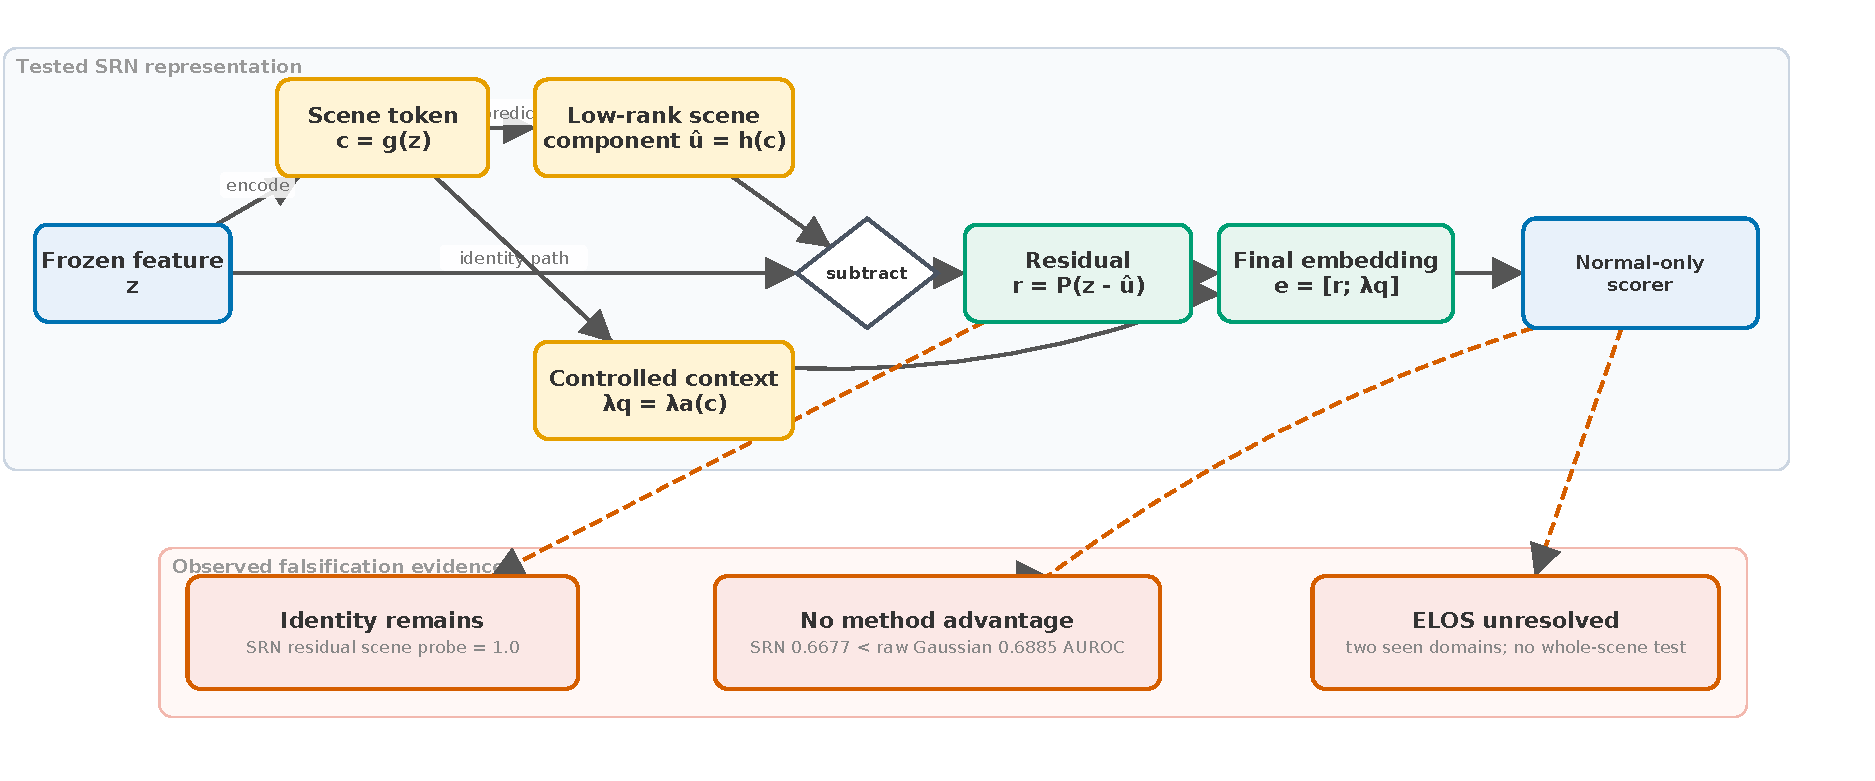
\includegraphics[width=\textwidth]{fig1_srn_falsification.pdf}
    \caption{The tested SRN representation and its falsification evidence. A low-rank component predicted from a scene token is removed, and a controlled context vector is optionally returned before normal-only scoring. On the two-seen-dataset diagnostic, identity remains perfectly decodable from the residual, raw Gaussian scoring is stronger, and the data cannot test genuine unseen-scene ELOS.}
    \label{fig:srn_falsification}
\end{figure*}

\section{Related Work}

\paragraph{Normal-only video anomaly detection.}
The established VAD setting fits a model of ordinary activity and evaluates deviations at test time. Early crowded-scene work combined dynamic texture models and discriminative saliency on UCSD data \citep{li2014anomaly}; Avenue was introduced with an efficient sparse-combination learning method \citep{lu2013abnormal}. Deep methods later used future-frame prediction to make abnormal motion or appearance difficult to predict \citep{liu2018future}. Memory-based approaches restrict reconstruction to learned normal prototypes, either by adding a memory to an autoencoder \citep{gong2019memorizing} or by coupling memory items to compactness and separateness losses \citep{park2020memory}. Our study does not compare end-to-end architectures. It freezes one general visual representation and asks whether low-capacity normality scorers fail because that representation contains dataset/camera nuisance information.

\paragraph{Scene dependence and evaluation.}
Anomalous behavior is contextual: an action may be ordinary in one location and exceptional in another. The Street Scene benchmark emphasized that single-scene and multi-scene formulations define different tasks and proposed criteria intended to better reflect practical event detection \citep{ramachandra2020street}. This observation creates a tension for scene invariance. Removing camera identity may improve transfer, but aggressive removal can also discard the location information that makes an event anomalous. SRN represents this tension explicitly through a constrained residual branch and a small context branch. Our evaluation therefore measures both dataset/camera decodability and anomaly ranking instead of interpreting lower scene accuracy alone as success.

\paragraph{Cross-domain VAD.}
Cross-domain work considers a detector trained on one collection and evaluated on another. For example, zxVAD studies cross-domain inference without target-domain adaptation and uses pseudo-anomalies plus a Normalcy Classifier module with relative-normalcy learning \citep{aich2023crossdomain}. That setting and ours are not directly comparable: zxVAD learns a video prediction model with auxiliary data, whereas we test normal-only scorers on a shared frozen cache and prohibit anomaly labels during selection. The methodological point we retain is that same-dataset and cross-dataset results answer different questions. We add a threshold distinction inside the latter: AUROC describes ordering after observing the full test curve, while a source-fixed threshold tests whether the numerical score scale transfers.

Multi-domain VAD has also been formalized through domain-generalization methods and broader benchmarks. Cho et al. formalize MDVAD, including leave-one-out training on multiple source domains and evaluation on an unseen target domain \citep{cho2024multidomain}, while MSAD introduces a 14-scenario multi-scenario benchmark \citep{zhu2024advancing}. Our two-dataset study cannot reproduce that evidential scope. Its role is a controlled falsification pilot for one residualization mechanism, not a multi-domain benchmark result.

\paragraph{Invariant and frozen representations.}
Domain-adversarial training uses a gradient-reversal layer to discourage domain prediction while optimizing a task representation \citep{ganin2016domain}. We include this construction as a generic residualization control and also apply it inside SRN. DINOv2 supplies the common frozen input because its self-supervised training targets broadly useful visual features \citep{oquab2024dinov2}. Freezing the backbone removes a major capacity confound: every scorer and residual variant receives exactly the same 384-dimensional frame feature. It also limits the conclusion. We study what a small residual module can do to one frozen image representation; we do not infer that temporal, object-centric, or end-to-end domain-generalization methods must behave similarly.

The closest evaluation precedent is Rashidi's cross-dataset audit of off-the-shelf frozen representations, including DINOv2, kNN, a Mahalanobis control, and false alarms per hour \citep{rashidi2026benchmark}. We do not claim novelty for auditing frozen-feature transfer. We instead add a predeclared source-threshold versus target-normal-calibration split and use a capacity-matched residualization matrix plus an independent identity probe to test whether a specific proposed mechanism repairs the observed shift.

\paragraph{Calibration and operating points.}
VAD papers commonly report frame AUROC, yet surveillance workloads care about low false-positive operation and alarm burden. Street Scene's evaluation critique motivates reporting explicit false-positive burden beyond frame AUROC; we therefore include false-alarm events per hour where frame rate is known \citep{ramachandra2020street}. We further separate two admissible thresholds. The strict threshold is estimated only from held-out source-normal scores. The calibrated threshold uses a predeclared set of target-normal videos and never uses target anomalies. Neither is the oracle threshold implicit in TPR at a selected point of the final test ROC curve. This separation is central to the empirical finding rather than a post-hoc metric choice.

\section{Problem Formulation and Tested Mechanism}
\label{sec:method}

\subsection{Normal-only transfer tracks}

Let $f$ be a frozen frame encoder and $z=f(x)\in\R^d$. Source training and validation sets contain only videos from the official training partitions. Final test labels are unavailable to feature extraction, representation learning, checkpoint selection, score fitting, and threshold selection. We distinguish two tracks.

In \emph{strict source-threshold transfer}, a scorer $A$ is fit on source-normal training embeddings and a threshold $\tau_{\mathrm{src}}$ is the empirical 99th percentile of source-normal validation scores. The target prediction is $\mathbb{1}[A(x)>\tau_{\mathrm{src}}]$. In \emph{target-normal calibration}, a separate, predeclared collection of target-normal training videos sets $\tau_{\mathrm{cal}}$ at the same quantile. This second track is adaptation to normal target data and is never called zero-shot. Target anomalies enter only the final evaluation of either fixed threshold.

Frame AUROC, average precision, and TPR at 1\% or 0.1\% FPR are also reported. The latter TPR values are \emph{oracle test-curve statistics}: test negatives locate the operating point on the final ROC curve. They measure ranking near the left edge but are not deployable thresholds.

\subsection{Scene-Residual Normality}

SRN starts from a frozen feature and predicts a removable component:
\begin{align}
    c &= g_{\phi}(z)\in\R^k, &
    \hat u &= h_{\psi}(c)\in\R^d, \\
    r &= P(z-\hat u), &
    q &= a_{\omega}(c), \\
    e &= [r;\lambda q].
\end{align}
Here $g_{\phi}$ is a linear 16-dimensional token, $h_{\psi}$ is a rank-8 linear factorization, and $P$ is a linear residual projection initialized to the identity. The optional context path has dimension eight and fixed weight $\lambda=0.25$. The scorer operates on $e$; the residual-only ablation operates on $r$.

For a normal frame $i$ with source identity $s_i$, the scene-prediction target $\mu_{s_i}$ is the mean frozen feature of that identity in the source training split. Training minimizes
\begin{equation}
\mathcal{L}=w_n\mathcal{L}_{\mathrm{compact}}
+w_p\lVert \hat u-\mu_s\rVert_2^2
+w_c\lVert\hat u\rVert_2^2
+w_r\lVert P-I\rVert_F^2
+\mathcal{L}_{\mathrm{scene}}^{\mathrm{GRL}},
\end{equation}
where the gradient-reversal term makes a scene classifier predict $s_i$ while reversing its gradient into the residual \citep{ganin2016domain}. The weights are $(w_n,w_p,w_c,w_r)=(0.05,1,0.01,1)$ and the gradient-reversal weight is $0.1$. This is deliberately a low-capacity test of the stated mechanism, not an architecture search.

For a batch $B$, the compactness term is
\begin{equation}
\mathcal{L}_{\mathrm{compact}}=\frac{1}{|B|D_e}
\sum_{i\in B}\left\lVert e_i-\operatorname{stopgrad}(\bar e_B)\right\rVert_2^2,
\qquad \bar e_B=\frac{1}{|B|}\sum_{i\in B}e_i,
\end{equation}
where $D_e$ is the embedding dimension. The normality head is fit after representation learning: kNN averages squared Euclidean distance to the five nearest training frames, the Gaussian head uses squared Mahalanobis distance with covariance shrinkage $0.1$, and the prototype head returns squared distance to the nearest of 32 centers learned by 20-step k-means.

\subsection{ELOS model selection and scope}

Episodic leave-one-scene-out (ELOS) cycles over source identities. At each epoch, one identity is excluded from the update; after the update, every source identity is treated in turn as held out, and the mean normal compactness relative to the remaining-source center selects a checkpoint. Only source-normal features are used. SRN without ELOS uses the ordinary source-normal validation score instead. ELOS without SRN is numerically identical to the raw representation because there is no learned representation checkpoint to select.

The joint experiment supplies only two identities---Ped2 and Avenue---and both appear during training and final testing. Thus it is a two-seen-domain diagnostic. It checks implementation behavior and source-normal selection, but it cannot establish whole-scene generalization. A legitimate ELOS claim requires multiple authoritative camera scenes and a final scene excluded from every training and selection operation.

\section{Experimental Protocol}
\label{sec:protocol}

\subsection{Data, representation, and splits}

Ped2 and Avenue originate in the corresponding UCSD and CUHK studies \citep{li2014anomaly,lu2013abnormal}. We use archives served by those official project pages and audit the decoded files locally. Ped2 contains 16 official training videos (2,550 frames) and 12 test videos (2,010 frames) at 10 FPS. Avenue contains 16 training videos (15,328 decoded frames) and 21 test videos (15,324 frames) at 25 FPS, with one aligned frame-mask file per test video. The Avenue project notes a few outliers in its training data; we retain the official partition without consulting anomaly annotations and therefore describe it as the official training split, not guaranteed anomaly-free data.

Every decoded frame is transformed by RGB conversion, bicubic resize to 256, center crop to $224\times224$, and ImageNet normalization. The official DINOv2 ViT-S/14 checkpoint \citep{oquab2024dinov2} produces one 384-dimensional class-token feature per frame. Checkpoint loading is strict. All methods share one immutable catalog of 35,212 features. Labels are joined only after each feature shard is complete.

Splits operate on whole videos. For the joint diagnostic, the first 12 training videos of each dataset form representation/scorer training; videos 13--14 form source-normal validation; videos 15--16 form the separately declared target-normal calibration set; all official test videos form final evaluation. The single-source cross-dataset caches similarly reserve whole source training videos for source validation and four target training videos for calibration. Assertions reject duplicate video keys, nonzero labels outside the test split, and declared dimensionality or dataset-identity mismatches.

\subsection{Comparisons and optimization}

Raw frozen features are scored with five-nearest-neighbor distance, shrinkage Gaussian/Mahalanobis distance, and distance to one of 32 normal prototypes. The mechanism matrix adds scene-mean subtraction, an adversarial residual, full SRN with ELOS, SRN without ELOS, ELOS without SRN, and SRN residual-only. A background-subtraction baseline is inapplicable because the cache has no label-free background feature; we do not synthesize one post hoc. Prototype and learned variants use seeds 13, 29, and 43. Gaussian and kNN are deterministic and run once. Learned representations use Adam for 30 epochs at learning rate $10^{-3}$; a bounded $10^{-4}$ diagnostic checks whether slower training changes the mechanism conclusion.

The prototype scorer is matched across SRN, its ablations, scene-mean subtraction, and the raw prototype control. Gaussian and kNN provide strong raw-feature reference points but do not share the prototype head. This distinction prevents the $0.0024$ SRN-versus-prototype delta from being presented as a win over the strongest scorer.

\subsection{Metrics and audit}

The main tables report frame micro AUROC, AUPRC, oracle test-curve TPR at 1\% and 0.1\% FPR, fixed-threshold recall and test-normal FPR, and the cross-domain q99 score ratio. Complete artifacts additionally contain macro-video AUROC, calibrated-track metrics, and false-alarm events per hour. False-alarm events are contiguous above-threshold normal runs after sorting by frame index and splitting on frame gaps. The independent scene probe is nearest-centroid identity classification: centroids are fit on held-out-from-test source training videos and evaluated on disjoint source-validation videos. It is not the adversarial training classifier.

Uncertainty for the joint comparison uses 500 hierarchical bootstrap replicates over test videos and, for stochastic methods, seeds. With two seen identities these intervals are descriptive, not population-level cross-scene confidence statements. A post-run independent integrity audit found no anomaly-label leakage, test-score normalization, failed-run selection, missing score artifacts, or frame-order bug. It classified the evidence as valid real-ground-truth pilot/diagnostic evidence with a scope warning. All reported runs executed on CPU.

ShanghaiTech Campus is the intended multi-scene ELOS stage, but it is absent from the audited experiment artifacts. We therefore report no ShanghaiTech result and make no unseen-scene claim; this omission does not invalidate the narrower Ped2/Avenue diagnostic.

\section{Results}
\label{sec:results}

\subsection{The tested residual does not improve the joint diagnostic}

\begin{table*}[t]
\centering
\caption{Joint two-seen-domain real-GT diagnostic. The protocol is not unseen-scene evaluation.}
\label{tab:main_results}
\small
\resizebox{\textwidth}{!}{%
\begin{tabular}{lrrrrrr}
\toprule
Method & AUROC $\uparrow$ & AUPRC $\uparrow$ & Oracle TPR@1\% $\uparrow$ & Oracle TPR@0.1\% $\uparrow$ & Source-thr. FPR $\downarrow$ & Scene probe \\
\midrule
Raw + Gaussian & 0.6885 & 0.5536 & 0.1082 & 0.0524 & 0.1686 & 1.000 \\
Raw + kNN & 0.6723 & 0.5025 & 0.0877 & 0.0321 & 0.2224 & 1.000 \\
Raw + prototype & 0.6653 & 0.5001 & 0.0857 & 0.0361 & 0.2058 & 1.000 \\
Scene mean + prototype & 0.6658 & 0.4985 & 0.0832 & 0.0360 & 0.2201 & 0.283 \\
Adversarial residual & 0.6657 & 0.5001 & 0.0854 & 0.0356 & 0.2056 & 1.000 \\
Full SRN + ELOS & 0.6677 & 0.5014 & 0.0880 & 0.0358 & 0.2054 & 1.000 \\
SRN without ELOS & 0.6657 & 0.4992 & 0.0864 & 0.0369 & 0.2045 & 1.000 \\
SRN residual only & 0.6665 & 0.5020 & 0.0838 & 0.0348 & 0.2050 & 1.000 \\
\bottomrule
\end{tabular}}
\vspace{1mm}\parbox{0.97\textwidth}{\footnotesize Raw Gaussian and kNN are deterministic (one run); stochastic prototype and learned rows use three seeds. Scene probe is held-video nearest-centroid dataset/camera accuracy. A value of 1.0 establishes decodability; below-chance binary accuracy is label-direction sensitive and is not interpreted as invariance. Oracle TPR columns are not deployable thresholds.}
\end{table*}


\Cref{tab:main_results,fig:method_comparison} compare methods on the joint two-seen-domain cache. Raw Gaussian is strongest by frame AUROC ($0.6885$) and AUPRC ($0.5536$); full SRN reaches $0.6677$ and $0.5014$. Their video-bootstrap intervals, $[0.5927,0.7994]$ and $[0.6066,0.7246]$, overlap broadly. Because Gaussian and SRN use different scorers, the stricter capacity-matched comparison is full SRN versus raw prototype. That delta is only $+0.002439\pm0.002456$ AUROC over three seeds, $+0.001272\pm0.002627$ AUPRC, and $-0.000311\pm0.001892$ oracle TPR at 0.1\% FPR. It does not support a practical or mechanistic advantage.

Scene-mean subtraction, adversarial residualization, and the learned ablations cluster near raw prototype. ELOS without SRN exactly equals raw prototype because the raw representation has no checkpoint. Removing ELOS or removing the context path changes AUROC by less than $0.0021$ relative to full SRN. The bounded lower-learning-rate diagnostic also fails to reduce scene decodability or improve the ordering. No component is justified by a consistent low-FPR gain.

\begin{figure*}[t]
    \centering
    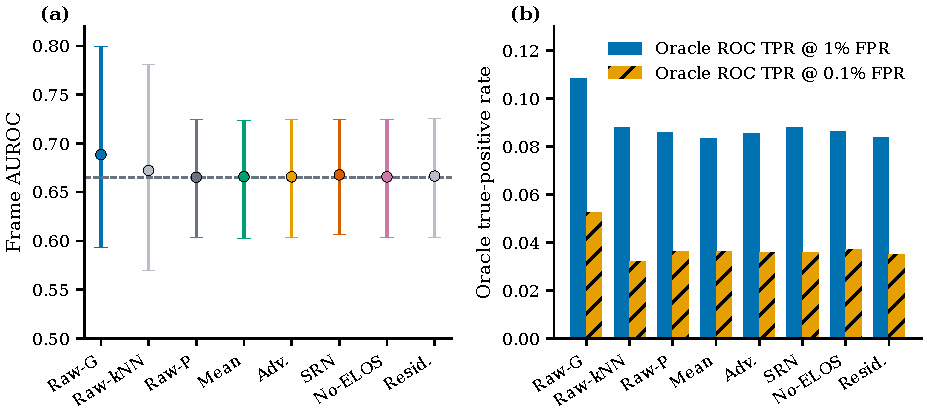
\includegraphics[width=\textwidth]{fig2_method_comparison.pdf}
    \caption{Joint two-seen-domain results. (a) Frame AUROC with descriptive 95\% hierarchical video/seed bootstrap intervals. The dashed line marks raw prototype. (b) Oracle test-curve TPR at 1\% and 0.1\% FPR; these bars use final test negatives to locate ROC operating points and are not deployable thresholds. Raw-G, Raw-P, Mean, Adv., No-ELOS, and Resid. denote raw Gaussian, raw prototype, scene mean, adversarial residual, SRN without ELOS, and SRN residual-only.}
    \label{fig:method_comparison}
\end{figure*}

\subsection{Source-fixed thresholds collapse across datasets}

\begin{table}[t]
\centering
\caption{Cross-dataset threshold transfer. Strict thresholds use source-normal validation only.}
\label{tab:threshold_transfer}
\small
\resizebox{\columnwidth}{!}{%
\begin{tabular}{llrrrrrr}
\toprule
Direction & Scorer & AUROC & Src. recall & Src. FPR & q99 ratio & Cal. recall & Cal. FPR \\
\midrule
Ped2$\to$Avenue & Gaussian & 0.3567 & 1.000 & 1.000 & 32.42 & 0.0038 & 0.0000 \\
Ped2$\to$Avenue & kNN & 0.3738 & 1.000 & 1.000 & 12.66 & 0.0000 & 0.0000 \\
Ped2$\to$Avenue & Prototype & 0.3759 & 1.000 & 1.000 & 13.22 & 0.0000 & 0.0000 \\
Avenue$\to$Ped2 & Gaussian & 0.6929 & 1.000 & 1.000 & 10.57 & 0.1620 & 0.0028 \\
Avenue$\to$Ped2 & kNN & 0.6541 & 1.000 & 1.000 & 6.50 & 0.0516 & 0.0028 \\
Avenue$\to$Ped2 & Prototype & 0.5353 & 1.000 & 1.000 & 6.68 & 0.0087 & 0.0018 \\
\bottomrule
\end{tabular}}
\vspace{1mm}\parbox{0.95\columnwidth}{\footnotesize Source thresholds are selected from source-normal validation only. q99 ratio is target-test-normal q99 divided by source-validation-normal q99. Target-calibrated thresholds use separately declared target-normal videos.}
\end{table}


The cross-dataset result is stronger than the small joint-method differences. Every scorer in both directions produces source-threshold test-normal FPR $1.0$ (\cref{tab:threshold_transfer,fig:threshold_transfer}). Consequently, the corresponding source-threshold recall of $1.0$ is an all-frames-flagged failure, not successful detection. Ped2-to-Avenue AUROC is also below chance for all three scorers ($0.3567$--$0.3759$). Avenue-to-Ped2 Gaussian reaches AUROC $0.6929$, demonstrating the central metric discrepancy: useful ordering can coexist with a completely unusable fixed threshold.

The numerical scale shift is large. Target-normal score q99 divided by source-normal validation q99 is $12.66$, $32.42$, and $13.22$ for Ped2-to-Avenue kNN, Gaussian, and prototype. In the reverse direction the ratios are $6.50$, $10.57$, and $6.68$. A 99th-percentile threshold calibrated on declared target-normal videos restores test-normal FPR to $0$--$0.0028$, but anomaly recall is only $0$--$0.0038$ for Ped2-to-Avenue and $0.0087$--$0.1620$ for Avenue-to-Ped2. Calibration changes the question and does not recover a strong detector here.

\begin{figure*}[t]
    \centering
    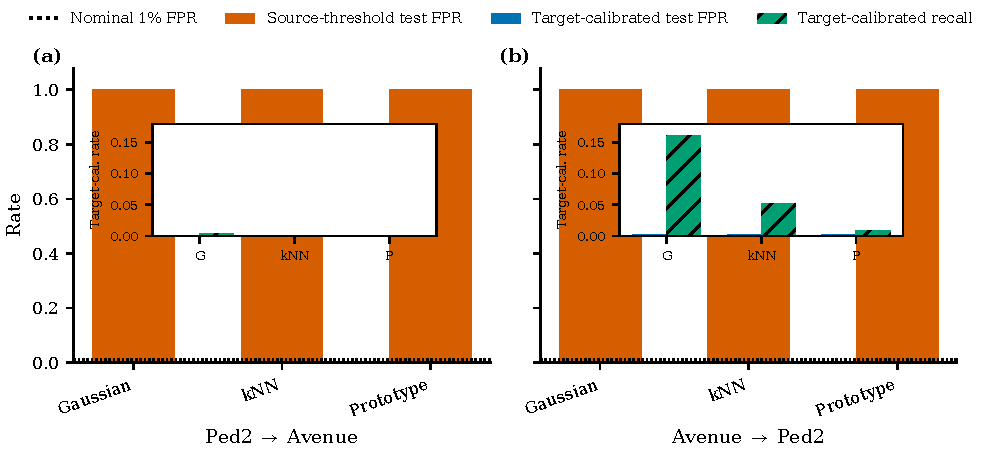
\includegraphics[width=\textwidth]{fig3_threshold_transfer.pdf}
    \caption{Cross-dataset threshold transfer for (a) Ped2 $\rightarrow$ Avenue and (b) Avenue $\rightarrow$ Ped2. Orange bars are test-normal FPR under a threshold fixed at 1\% source-normal validation FPR. Insets show the separate target-normal calibration track. All source thresholds flag every target normal frame.}
    \label{fig:threshold_transfer}
\end{figure*}

\subsection{Within-dataset checks do not predict transfer}

Within-dataset checks confirm that the pipeline can produce meaningful rankings. Ped2 raw Gaussian obtains AUROC $0.8982$, AUPRC $0.9780$, source-threshold recall $0.6238$, and test-normal FPR $0.0028$. Avenue is harder: the three-seed raw prototype obtains AUROC $0.6197\pm0.0008$, AUPRC $0.4235$, recall $0.1431\pm0.0056$, and FPR $0.0208\pm0.0014$. These results are engineering sanity checks, not state-of-the-art comparisons. Their contrast with cross-dataset FPR $1.0$ shows that successful within-dataset calibration does not imply score-scale transfer.

\section{Diagnostics, Interpretation, and Limitations}
\label{sec:diagnostics}

\paragraph{The identity-removal mechanism failed.}
The independent two-way dataset/camera probe scores $1.000$ on raw features, adversarial residuals, and the full SRN residual. Thus the learned residual leaves the measured identity accessible to nearest-centroid classification. Scene-mean subtraction changes probe accuracy to $0.283$, but a below-chance binary accuracy is label-direction sensitive and is not evidence of invariance; we therefore draw no identity-removal conclusion from that row. It also does not improve anomaly AUROC over the matched raw prototype. Identity suppression and anomaly detection are separate requirements, and neither result alone validates SRN.

\paragraph{Optimization is not the parsimonious explanation.}
Source-normal validation chooses the earliest post-update checkpoint for the main trainable variants. This could indicate a poorly aligned objective, so we ran one controlled diagnostic at learning rate $10^{-4}$. It permits later adversarial checkpoint selection but leaves the SRN probe at $1.000$ and AUROC near $0.668$. Broader tuning would use the same two datasets repeatedly and risks converting a mechanism test into test-specific architecture search. We stop rather than tune on final anomaly labels or select the best seed.

\paragraph{Threshold failure and mechanism failure are distinct.}
The raw-score q99 ratios establish a large source-to-target scale shift. That evidence supports the nuisance premise: frozen features and their normality scores are dataset/camera dependent. It does not identify scene-predictable feature subtraction as the remedy. Conversely, the joint SRN comparison is a mechanism diagnostic with both identities seen in training, so it cannot demonstrate or refute performance on a genuinely unseen camera scene. The safe conclusion is narrow: the premise motivates further calibration research, while the tested low-capacity residualization mechanism has no supported advantage on Ped2/Avenue.

\paragraph{Dataset and representation limits.}
Ped2 and Avenue differ in camera, resolution, frame rate, content, and anomaly definitions. Cross-dataset labels therefore measure both covariate and task shift. Avenue's official training partition has documented outliers that we retain without label-based filtering. The frame encoder is image-based, so it lacks explicit motion and object tracks. We apply no temporal smoothing; false-alarm events per hour are consequently diagnostic rather than an optimized alarm policy. The joint probe uses dataset identity as a camera/scene surrogate, not within-dataset camera labels.

\paragraph{Statistical and baseline limits.}
Only two dataset identities are available, Gaussian and kNN are deterministic one-run baselines, and three seeds cannot establish broad stability. Bootstrap intervals resample observed test videos, not new scenes. Background subtraction is omitted because no label-free background cache exists. We do not compare end-to-end prediction, object-centric, skeleton, language-model, or pseudo-anomaly systems, so the tables are controlled falsification experiments rather than a leaderboard.

\paragraph{ELOS remains unresolved.}
The implementation performs source-normal episodic selection, but the audited data do not contain a final identity unseen throughout training and model selection. ShanghaiTech is not part of the experiment artifacts. We therefore make no ELOS generalization claim. Reconsidering SRN requires an authoritative multi-scene cache, a preregistered held-out-scene protocol, a substantial reduction in independent residual scene-probe accuracy, and non-degraded source-fixed low-FPR detection. Until then, the current evidence does not justify further tuning of this SRN formulation.

\section{Conclusion}

This study tested a specific explanation for poor normal-only transfer: scene-predictable components in frozen visual features harm anomaly scoring, and low-capacity residualization can remove them. The first part of that premise receives bounded support. Ped2/Avenue score scales shift so severely that source-normal thresholds flag every target normal frame, even when AUROC remains nontrivial. The proposed remedy does not. Full SRN trails raw Gaussian scoring, barely changes its matched prototype head, and leaves dataset/camera identity perfectly decodable.

The result is a mechanism falsification, not evidence that scene dependence is irrelevant or that all invariant VAD methods fail. Genuine unseen-scene ELOS remains untested because no multi-scene asset is present in the audited experiment set. A future study should first secure such data, freeze the split and thresholds, and require simultaneous success on identity suppression, event retention, and source-fixed low-FPR behavior. The current evidence does not justify further tuning of this SRN formulation.

\paragraph{Reproducibility and broader impact.}
The repository records dataset and checkpoint hashes, whole-video split identities, extraction preprocessing, all configurations and seeds, per-frame score artifacts, audit results, and figure-generation scripts. VAD errors can burden operators or miss harmful events; the failure of source-fixed thresholds reported here is a reason to validate calibration under deployment shift, not to deploy the tested system.


\bibliography{references}
\bibliographystyle{iclr2026_conference}

\appendix
\section{Additional Protocol and Results}

\subsection{Exact split sizes}

\begin{table}[h]
\centering
\caption{Whole-video split sizes, shown as videos/frames. Source and calibration partitions contain official training videos only; final test partitions are the complete official test splits.}
\label{tab:splits}
\small
\begin{tabular}{lrrrr}
\toprule
Track & Train & Source val. & Target cal. & Test \\
\midrule
Joint seen & 24/15,775 & 4/1,206 & 4/897 & 33/17,334 \\
Ped2$\to$Avenue & 12/1,920 & 4/630 & 4/5,873 & 21/15,324 \\
Avenue$\to$Ped2 & 12/13,855 & 4/1,473 & 4/600 & 12/2,010 \\
\bottomrule
\end{tabular}
\end{table}

\subsection{Within-dataset sanity checks}

\begin{table}[h]
\centering
\caption{Within-dataset raw-feature sanity checks. Prototype means use three seeds, with selected standard deviations shown; deterministic rows use one run. Oracle TPR uses the final test ROC curve.}
\label{tab:within}
\small
\begin{tabular}{llrrrr}
\toprule
Dataset & Scorer & AUROC & AUPRC & Oracle TPR@1\% & Source-thr. FPR \\
\midrule
Ped2 & Gaussian & 0.8982 & 0.9780 & 0.6845 & 0.0028 \\
Ped2 & kNN & 0.8806 & 0.9741 & 0.6614 & 0.0000 \\
Ped2 & Prototype & $0.8802\pm0.0018$ & 0.9740 & 0.6608 & 0.0000 \\
Avenue & Gaussian & 0.6109 & 0.4183 & 0.1061 & 0.0158 \\
Avenue & kNN & 0.6148 & 0.4155 & 0.1032 & 0.0196 \\
Avenue & Prototype & $0.6197\pm0.0008$ & 0.4235 & 0.1043 & $0.0208\pm0.0014$ \\
\bottomrule
\end{tabular}
\end{table}

\subsection{Artifact and leakage gates}

Each feature cache contains feature dimension, dataset identity, scene/video key, split, label, FPS, and frame index arrays plus a JSON provenance sidecar. The loader requires a dataset identifier, verifies array lengths and finite features, rejects nonzero anomaly labels outside the final test split, and requires whole-video separation when configured. The feature-catalog and DINOv2-checkpoint SHA-256 prefixes are \texttt{9d048d0fadeb9d} and \texttt{b938bf1bc15c}; the complete hashes and source URLs are retained in the project provenance file.

All final run directories contain a configuration snapshot, structured result JSON, per-frame compressed score arrays, and logs. Expected matrix row counts match observed outputs. No failed seed was removed. The target-normal calibration split never contains test anomalies and is reported separately from strict source-threshold transfer.

\subsection{Alarm counting}

For each normal test video, frames are sorted by frame index. A false-alarm event begins when the score crosses above the fixed threshold after a below-threshold frame or an index gap. Event counts are divided by total normal-frame duration using the dataset FPS. This prevents shuffled result rows or discontinuous normal intervals from merging unrelated alarms.

\subsection{Evidence classes}

The frozen-feature extractor, cache guards, tests, and within-dataset results provide engineering validation. The Ped2/Avenue cross-dataset and joint-seen results are real-ground-truth pilot evidence. They are formal for the exact stored splits and metrics but insufficient for population-level or unseen-scene claims. No result in this paper supports general SRN efficacy or ELOS generalization.

\end{document}
